\chapter{Geometria/Relações (1º Bimestre)}

\section{Pontos e retas}

The pontos de um plano can be described using coordinates $(x,y)$ in a cartesian
coordinate system. The distance between two points of coordinates
$(x_1,y_1)$ and $(x_2,y_2)$ is given by the Pitagora theorema:
%%
$$d = \sqrt{{(x_2-x_1)}^2 + {(y_2-y_1)}^2}$$
%%
The punto medio of $(x_1,y_1)$ and $(x_2,y_2)$ is
%%
$$
(x_3,y_3) = \left(\frac{x_1+x_2}{2}, \frac{y_1+y_2}{2}\right)
$$
%%
Given  two points of coordinates $(x_1,y_1)$, $(x_2,y_2)$ and a third
points $(x_3,y_3)$ distinct of the two others, then the three points are
aligned iff there is a coefficient $\lambda$ such that
%%
$$
\begin{gathered}
x_3 - x_1 = \lambda\left(x_3-x_2\right) \\
y_3 - y_1 = \lambda\left(y_3-y_2\right)
\end{gathered}
$$
%%
This implies the following relation for the determinant:
%%
$$
\begin{vmatrix}
x_3 - x_1 & x_3-x_2 \\
y_3 - y_1 & y_3-y_2
\end{vmatrix} = 0
$$
%%
which is also obviously true if $(x_3,y_3) = (x_1,y_1)$ and
$(x_3,y_3) = (x_2,y_2)$.

Given coefficients $a,b,c$ we consider the set of points $(x,y)$ satisfying
the equation $ax + by + c = 0$. If $a=b=0$, it is either the whole plano
or the empty set, according to whether $c = 0$ or not. If $a \neq 0$ and
$b = 0$, the equation can be written $x = -\frac{c}{a}$ which correspond to
a vertical line. Similarly, $a=0$ and $b=0$ gives the equation of a
horizontal line $y = -\frac{c}{b}$. Finally, if $a, b \neq 0$, the equation is
$y = -\frac{a}{b} x - \frac{c}{b}$
which corresponds to the graph (reta) of a linear function that is neither
vertical nor horizontal.
Conversely, if we consider uma reta given by two distinct points
$(a,b)$, $(c,d)$ then the set of points $(x,y)$ on it satisfies the equation
%%
$$
\begin{vmatrix}
x - a & x-c \\
y - b & y-d
\end{vmatrix} = Ax + By + C = 0
$$
%%
where $A = b-d$, $B = c-a$ and $C = \begin{vmatrix}
a & c \\
b & d
\end{vmatrix} = ad-bc$ and $(A,B) \neq (0,0)$.

We now consider two retas of equations $a_1x + b_1y+c_1=0$ and
$a_2x + b_2y+c_2=0$. We have $(a_1,b_1) \neq 0 \neq (a_2,b_2)$.
A point $(x,y)$ on the intersection of these two retas
satisfy the matricial equation
%%
$$
\begin{pmatrix}
  a_1 & b_1 \\
  a_2 & b_2
\end{pmatrix}
\begin{pmatrix}
  x \\
  y
\end{pmatrix}
=
\begin{pmatrix}
  -c_1 \\
  -c_2
\end{pmatrix}
$$
%%
There is a unique solution (retas secantes) iff
$\begin{vmatrix}
a_1 & b_1 \\
a_2 & b_2
\end{vmatrix} = a_1b_2 - b_1a_2 \neq 0$ and the intersection point is
$$\begin{pmatrix}
  x \\
  y
\end{pmatrix} =
\frac{1}{a_1b_2 - b_1a_2}
\begin{pmatrix}
  b_2 & -b_1 \\
  -a_2 & a_1
\end{pmatrix}\begin{pmatrix}
  c_1 \\
  c_2
\end{pmatrix} = \begin{pmatrix}
  \frac{b_2c_1-b_1c_2}{a_1b_2 - b_1a_2} \\
  \frac{a_1c_2-a_2c_1}{a_1b_2 - b_1a_2}
\end{pmatrix}$$
We can prove that the retas are orthogonal iff
$a_1a_2+b_1b_2=0$ (see for example exercise 2).

If $\begin{vmatrix}
a_1 & b_1 \\
a_2 & b_2
\end{vmatrix} = 0$ then the retas are either parallel or equal. Equivalently,
$(a_1,b_1)$ and $(a_2,b_2)$ are proportional.
Suppose that they are equal. By the analysis of the coefficient
$a_1 = 0$ iff $a_2 = 0$ iff the retas are horizontal and in that case
the equation is $y = -\frac{c_1}{b_1} = \frac{c_2}{b_2}$.
Similarly, $b_1 = 0$ iff $b_2 = 0$ iff the retas are vertical
and in that case
the equation is $x = -\frac{c_1}{a_1} = \frac{c_2}{a_2}$.
Now suppose $a_1, b_1, a_2, b_2 \neq 0$. If $c_1 = 0$ then the point $(0,0)$
satisfies the first equation so it must satisfy the second, that is $c_2 = 0$
and similarly if $c_2=0$ then $c_1=0$. In that case, the point
$\left(-\frac{b_1}{a_1}, 0\right)$ satisfies the first equation so
it must satisfy the second and we get $\frac{a_2}{a_1} = \frac{b_2}{b_1}$.
Finally, if moreover $c_1,c_2 \neq 0$ the point
$\left(-\frac{c_1}{a_1}, 0\right)$ satisfies the first equation so it must
satisfy the second one, from which we obtain
$\begin{vmatrix}
a_1 & c_1 \\
a_2 & c_2
\end{vmatrix} = 0$. Similarly, we have $\begin{vmatrix}
b_1 & c_1 \\
b_2 & c_2
\end{vmatrix} = 0$. We conclude that
$\frac{a_2}{a_1} = \frac{b_2}{b_1} = \frac{c_2}{c_1}$. We can summarize all the
cases by saying that the retas are equal if
$(a_1,b_1,c_1)$ and $(a_2,b_2,c_2)$ are proportional and the converse is obvious.

La distância de um punto $A=(x_1,y_1)$ a uma reta $\mathcal R$
de equação $ax+by+c=0$
is the minimal distance between $A$ and a point of $B$ of the reta.
Such a point $P$ where the minimum is reached is unique: it is the point
of the reta such that $(AB) \perp \mathcal R$. Using the previous
characterization of orthogonality, we can easily find the coordinate of $P$
(see Exercício 3 for an example).

\subsection*{Exercício 1}

\begin{enumerate}
\item What can you say about the retas of equations $x=2$ and $y=1$.
  What is the coordinate of their intersection $A$?
\item Let $B,C$ be the points of coordinates $(2,-2)$ and $(6,1)$.
  Determine the length $BC$.
\item What are the coordinates of the middle $O$ of $[BC]$?
\item Verify that $OA=OB=OC$.
\item Let $D$ be the point of coordinate $\left(0,\frac{5}{2}\right)$.
  Show that $D,A,O$ are aligned.
\item Give an equation for the reta $(BC)$?
\item Give an equation for the reta ${\mathcal R}_1$
  orthogonal to $(BC)$ passing by $D$?
\item Give an equation for the reta ${\mathcal R}_2$ parallel to
  $(BC)$ passing by $D$, using the condition for two retas to be parallel.
\item Verify that ${\mathcal R}_1 \perp {\mathcal R}_2$ from these equations.
\end{enumerate}

\subsection*{Exercício 2}

\begin{enumerate}
\item Let $a_1x+b_1y=c_1$ and $a_2x+b_2y+c_2$ be two retas.
  Suppose that $a_1=0$ or $b_1=0$.
  Show that the retas are orthogonal iff $a_1a_2+b_1b_2=0$.
\item We consider three distinct points
  $A={(x_1,y_1)}, B={(x_2,y_2)}, C={(x_3,y_3)}$.
  Determine the lengths of the sides of the triangle $ABC$.
\item Expand the expression ${BC}^2 - {AB}^2 - {AC}^2$.
\item Show that $ABC$ is rectangle in $A$
  iff ${(y_2-y_1)}{(y_3-y_1)}+{(x_2-x_1)}{(x_3-x_1)} = 0$.
\item Verify that $(AB)$, $(AC)$ have respective equations
  %%
  $${(y_2 - y_1)} x + {(x_1 - x_2)} y + {(x_2y_1 - y_2x_1)} = 0$$
  $${(y_3 - y_1)} x + {(x_1 - x_3)} y + {(x_3y_1 - y_3x_1)} = 0$$
  %%
\item We now consider retas secantes of equations
  $a_1x+b_1y=c_1$ and $a_2x+b_2y+c_2$ with $a_1,b_1,a_2,b_2 \neq 0$.
  Let $x_1 = \frac{b_2c_1-b_1c_2}{a_1b_2 - b_1a_2}$ and
  $y_1 = \frac{a_1c_2-a_2c_1}{a_1b_2 - b_1a_2}$
  be the coordinates of the intersection point.
  Let $y_2=a_1+y_1$, $x_2=-b_1+x_1$, $y_3=a_2+y_1$
  and $y_3=-b_2+x_1$. Verify that ${(x_2y_1 - y_2x_1)} = c_1$ and
  ${(x_3y_1 - y_3x_1)} = c_2$.
\item Show that the retas are orthogonal iff
  $a_1a_2+b_1b_2=0$.
\end{enumerate}

\subsection*{Exercício 3}

We consider the reta $\mathcal R$ of equation $y+2x+3=0$ and the point $P$
of coordinate $(4,5)$.

\begin{enumerate}
\item Verify that $P \notin \mathcal R$.
\item Express the distance between $P$ and a point $(x,y)$ of
  $\mathcal R$ as $d=\sqrt{ax^2+bx+c}$ for some constants $a,b,c$.
\item Determine the point $Q \in \mathcal R$ of $(x,y)$ for which this distance
  is minimal.
\item For any point $S \neq P$ of coordinates $(x_1,y_1)$ determine an
  equation for $(PS)$.
\item Show that $(PS) \perp \mathcal R$ iff $-x_1+2y_1-6=0$.
\item Find the point $S \in \mathcal R$ such that $(PS) \perp \mathcal R$
\item What do you notice?
\end{enumerate}

\section{Equações e inequações lineares}

Given any $(a,b) \neq 0$ then any coefficient $c$ allows to define uma reta
with the equation $ax+by+c=0$. As we have previously seen, for different
values of $c$ we obtain parallel retas. When $c$ varies, these paralell retas
will cover the whole plano, that is for any point $(x_1,y_1)$, there is some
$c_1$ such that $ax_1+by_1+c_1=0$.

Now if we fix $c_0$, the reta $ax+by+c_0=0$ splits the plano into two parts:
the points $(x_1,y_1)$ for which $ax_1+by_1 + c_0 > 0$ (equivalently
for which $c_1 < c_0$)
and those for which $ax_1+by_1 + c_0 < 0$ (equivalently for which $c_1 > c_0$)
corresponding to the semi-plano on each side of the reta.

Now a set of inequations of the forms
$a_ix+b_iy + c_i \geq 0$, $a_ix+b_iy + c_i \leq 0$,
$a_ix+b_iy + c_i > 0$ and $a_ix+b_iy + c_i < 0$ deliminate several semi-planos
and their intersection correspond to the points that are solutions to this
system of inequations.

\subsection*{Exercício 4}

We mix a liquid $A$ of density $1000 \text{kg}.\text{m}^{-3}$ with a liquid
$B$  of density $1500 \text{kg}.\text{m}^{-3}$ in a recipient of maximal
capacity $6\text{m}^3$. We consider quantities $x \geq 1 \text{m}^{3}$ of $A$
and $y \geq 2 \text{m}^{3}$ of $B$ such that the total mass of the mixture
does not exceed $7600\text{kg}$. What are the acceptable values for $x,y$?
Draw it on a schema.

\section{Circunferências e Cônicas}

The circunferência of center $(x_1,y_1)$ and radius $R$ is the set of points
$(x,y)$ at distance $R$ of $(x_1,y_1)$. We saw that this distance was
$d = \sqrt{{(x-x_1)}^2 + {(y-y_1)}^2}$ so the equation of the
circunferência is
%%
$${(x-x_1)}^2 + {(y-y_1)}^2 = R^2$$
%%
or equivalently
%%
$${\left(\frac{x-x_1}{R}\right)}^2 + {\left(\frac{y-y_1}{R}\right)}^2 = 1$$
%%
\begin{center}
  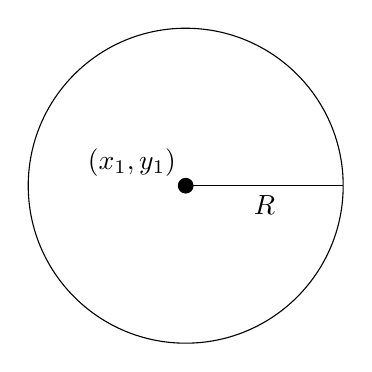
\begin{tikzpicture}
    \draw (0,0) circle(2);
    \fill(0,0) circle(.1)node[above left]{$(x_1,y_1)$};
    \draw(0,0) -- (1,0) node[below]{$R$} -- (2,0);
  \end{tikzpicture}
\end{center}
We can consider the case $R=1$ and stretch this unit circle horizontally by a
an arbitrary factor $a$ and vertically by another arbitrary factor $b$.
We obtain the reduced equation of an
ellipse of center $(x_1,y_1)$ and axis parallel to those of the cartesian
coordinate system, of demi-axis $a$ and $b$.
%%
$${\left(\frac{x-x_1}{a}\right)}^2 + {\left(\frac{y-y_1}{b}\right)}^2 = 1$$
%%
\begin{center}
  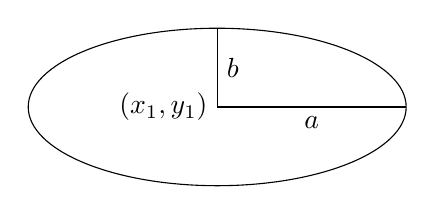
\begin{tikzpicture}[xscale=1.2,yscale=.5]
    \draw (0,0) circle(2);
    \draw(0,0) node[left]{$(x_1,y_1)$};
    \draw(0,0) -- (1,0) node[below]{$a$} -- (2,0);
    \draw(0,0) -- (0,1) node[right]{$b$} -- (0,2);
  \end{tikzpicture}
\end{center}
A similar equation gives an hyperbola:
%%
$${\left(\frac{x-x_1}{a}\right)}^2 - {\left(\frac{y-y_1}{b}\right)}^2 = 1$$
%%
\begin{center}
  \begin{tikzpicture}
    \fill(0,0) circle(.1);
    \draw(0,0) node[left]{$(x_1,y_1)$};
    \draw (-3.703393523556585,-1.1752011936438014) --(-3.4394073250770587,-1.0265167257081753) --(-3.209843871131627,-0.888105982187623) --(-3.012405613514263,-0.7585837018395334) --(-2.845116523781442,-0.6366535821482412) --(-2.7063023164953135,-0.5210953054937474) --(-2.594573692412292,-0.4107523258028155) --(-2.5088124339092652,-0.3045202934471426) --(-2.448160213485782,-0.20133600254109402) --(-2.4120100033339282,-0.10016675001984403) --(-2.4,0) --(-2.4120100033339282,0.10016675001984403) --(-2.448160213485782,0.20133600254109402) --(-2.5088124339092652,0.3045202934471426) --(-2.594573692412292,0.4107523258028155) --(-2.7063023164953135,0.5210953054937474) --(-2.845116523781442,0.6366535821482412) --(-3.012405613514263,0.7585837018395334) --(-3.209843871131627,0.888105982187623) --(-3.4394073250770587,1.0265167257081753) --(-3.703393523556585,1.1752011936438014)
    (3.703393523556585,-1.1752011936438014) --(3.4394073250770587,-1.0265167257081753) --(3.209843871131627,-0.888105982187623) --(3.012405613514263,-0.7585837018395334) --(2.845116523781442,-0.6366535821482412) --(2.7063023164953135,-0.5210953054937474) --(2.594573692412292,-0.4107523258028155) --(2.5088124339092652,-0.3045202934471426) --(2.448160213485782,-0.20133600254109402) --(2.4120100033339282,-0.10016675001984403) --(2.4,0) --(2.4120100033339282,0.10016675001984403) --(2.448160213485782,0.20133600254109402) --(2.5088124339092652,0.3045202934471426) --(2.594573692412292,0.4107523258028155) --(2.7063023164953135,0.5210953054937474) --(2.845116523781442,0.6366535821482412) --(3.012405613514263,0.7585837018395334) --(3.209843871131627,0.888105982187623) --(3.4394073250770587,1.0265167257081753) --(3.703393523556585,1.1752011936438014);
  \end{tikzpicture}
\end{center}
Finally, we have already seen that a parabola can be express as an expression
of the form
$y = \frac{1}{4p} \left(x-x_0\right)^2 + y_0$ corresponding to the graph
of a cuadratic function. $x=x_0$ is the axis of symmetry, $(x_0,y_0)$ the
vertex of the parabola and $p$ another parameter (see Exercício 9 for
the interpretation). Translating the center of the coordinate system,
this can be reduced to the canonical form $x^2 = 4py$.

We consider uma circunferência of center $(x_1,y_1)$ and radius $R$. There
are three relative position for uma reta at distance $d$ of the center:

\begin{enumerate}
\item If $d<R$ then the reta and circunferência are secantes.
\item If $d=R$ then the reta is tangente to la circunferência.
\item If $d=R$ then the reta and circunferência do not intersect.
\end{enumerate}

\begin{center}
 \begin{tikzpicture}
   \draw[color=blue] (0,0) circle(.1)[fill=blue];
   \draw[color=blue] (0,0) circle(2) (2,0);
   \draw[color=red] (-2,-2) -- (-1,3) node[above right] {$d<R$};
   \draw[color=red] (3,-3) -- (5,3) node[above right] {$d>R$};

   \begin{scope}[rotate around={-10:(0,0)}]
   \draw[color=blue] (2,0) circle(.1)[fill=blue];
   \draw[color=red] (2,-4) -- (2,4) node[above right] {$d=R$};
   \draw[color=orange](1.8,0) -- (1.8,.2) -- (2,.2);
   \draw[color=orange](0,0) -- (1,0) node[below]{$R$} -- (2,0);
   \end{scope}

 \end{tikzpicture}
\end{center}

If la reta has equation $ax+by+c=0$ then we can express one of $x$ or $y$
in function of the other and reinjecting in the equation of the circle
${(x-x_1)}^2 + {(y-y_1)}^2 = R^2$ we obtain a second order equation that we
can solve to find the intersection point.

Given two circle of centers $A=(x_1,y_1)$ and $B=(x_2,y_2)$ such that
$A\neq B$ and respective
radius $R_1,R_2$, we consider the set of points $P=(x,y)$
such that ${AP}^2 - R_1^2 = {BP}^2 - R_2^2$. Using the formula for the
distance of two points, we can simplify this equality as
${2{(x_2-x_1)}} x + {2{(y_2-y_1)}} y + {(x_1^2+y_1^2-R_1^2-x_2^2-y_2^2+R_2^2)}
= 0$. Hence we obtain the a line called the radical axis of the two circles.
We note that if $P$ is one the intersection of the two circles then
$AP = R_1$ and $BP = R_2$ so $P$ is on the radical axis. Conversely,
if $P$ is on one of the circle (say the first one) and on the radical axis
then $AP = R_1$ and ${AP}^2 - R_1^2 = {BP}^2 - R_2^2$ implies
$BP = R_2$ that is $P$ is on the other circle. As a consequence to determine
the relative position of the two circle, it is enough to consider the
relative intersection of one of the circle with the radical axis.

\subsection*{Exercício 5}

\begin{enumerate}
\item Show that the curve of equation $y^2-4y+x^2-2x+2 = 0$ is uma
  circunferência.
\item  What is the relative position of this circunferência with the
  reta of equation $3y-2x+2=0$?
\item With the reta of equation $x + y - \sqrt{3} - 3 = 0$?
\item With the reta of equation $x - 1 +\sqrt{3} = 0$?
\end{enumerate}

\subsection*{Exercício 6}

\begin{enumerate}
\item Show that the curves of equations
  $y^2-6y+x^2-10x+33=0$ and
  $y^2-6y+x^2-14x+57=0$ are circunferências and determine the centers
  and radius.
\item What is the equation of the radical axis of these two circunferências?
\item Deduce the relative position of the two circunferências.
\item Same questions for the curves of equations
  $y^2-2y+x^2=0$ and $y^2-6y+x^2-4x+8=0$.
\end{enumerate}

\subsection*{Exercício 7}

Identify the curves given by the following equations

\begin{enumerate}
  \item ${(x+y)}^2 - {(x-1)}^2 = y^2 + 2xy$
  \item $4y^2-24y-x^2+2x+39=0$
  \item $y^2-10y+x^2-14x+7=0$
  \item $y^2-2y-441x^2+50=0$
  \item $y - 2x^2-4x-5=0$
  \item $xy = 1$ (rotate the coordinate system by $\frac{\pi}{4}$, that
    is set $u = \frac{\sqrt{2}}{2}\left(x+y\right)$ and
    $v = \frac{\sqrt{2}}{2}\left(y-x\right)$).
\end{enumerate}

\subsection*{Exercício 8}

We consider the parameteric definition
$\{ (x(t), y(t)) : t \in \mathbb R \}$ below. Determine an equation in $x,y$
for these curves and identify them.

\begin{enumerate}
\item $x(t) = a + t b$ and $y(t) = c + t d$ for some constants $a,b,c,d$
  such that $(b,d) \neq (0,0)$.
\item $x(t) = a\cos{(t)}$ and $y(t) = b\sin{(t)}$ for some
  constants $a,b > 0$.
\item $x(t) = a \frac{e^t+e^{-t}}{2}$ and $y(t)= b \frac{e^t-e^{-t}}{2}$
  for some constants $a,b > 0$.
\item $x(t) = \frac{1}{4p}t^2$ and $y(t) = t$ for some constant $p$.
\end{enumerate}

\subsection*{Exercício 9}

Let $p$ be a constant.

\begin{enumerate}
\item Let $F=(p,0)$. Express the distance $FP$ for any point $P=(x,y)$.
\item Let $D$ be the line of equation $x = -p$. Determine the distance from
  any point $P=(x,y)$ to $D$.
\item What is the set of points for which these two distances are equal?
\end{enumerate}

\subsection*{Exercício 9}

Let $p$ be a constant.

\begin{enumerate}
\item $\sqrt{{(x-p)}^2+y^2}$
\item The point $Q \in D$ such that $PQ$ is minimal (or equivalently such
  that $(PQ) \perp D$) is $Q=(-p,y)$.
  So the distance from $P$ to $D$ is $\sqrt{{(x+p)}^2+{(y-y)}^2} = {|x+p|}$
\item $\sqrt{{(x-p)}^2+y^2} = |x+p|$ or equivalently
  $x^2-2xp+p^2+y^2=x^2+2xp+p^2$ that is
  $y^2=4px$. Hence this is the parabola of axis the $x$-axis, vertex $(0,0)$
  and parameter $p$.
\end{enumerate}

\section{Solução do Exercícios}

\subsection*{Exercício 1}

\begin{enumerate}
\item $x=2$ is vertical and $y=1$ is horizontal. They are perpendicular
  and intersect at point $A$ of coordinate $(2,1)$.
\item $BC= \sqrt{{(6-2)}^2 + {(1+2)}^2} = 5$.
\item
  $O$ has coordinate $\left(\frac{6+2}{2}, \frac{1-2}{2}\right)=
  \left(4, -\frac{1}{2}\right)$
\item By definition $OB=OC=\frac{BC}{2}=\frac{5}{2}$.
  Moreover $OA=\sqrt{{(2-4)}^2 + {(1+\frac{1}{2})}^2}=\frac{5}{2}$
\item For example, we have
  $$
\begin{vmatrix}
0 - 4 & 0-2 \\
\frac{5}{2} + \frac{1}{2} & \frac{5}{2}-1
\end{vmatrix} =
\begin{vmatrix}
-4 & -2 \\
3 & \frac{3}{2}
\end{vmatrix} = -6 + 6 = 0
$$
\item $2=x_B \neq x_C = 6$ so $(BC)$ is not vertical and we can write
  in the form $y = ax+b$ for some constants $a,b$.
  We have $-2=2a+b$ and $1=6a+b$ so $a = \frac{1+2}{6-2}  = \frac{3}{4}$
  and $b = -2 - 2 \times \frac{3}{4} = -\frac{7}{2}$.
  Finally one equation is
  $-\frac{3}{4} x + y + \frac{7}{2} = 0$. All other equations can be obtained
  by multiplying the coefficients by a same nonzero factor, for example
  $-3x+4y+14=0$.

\item It is not horizontal so can be written
  $x + cy + d =0$ where $1 \times c - \frac{3}{4} \times 1 = 0$ that is
  $c = \frac{3}{4}$. Evaluating at $(x,y)=\left(0,\frac{5}{2}\right)$ we find
  $d = -\frac{3}{4} \times \frac{5}{2} = -\frac{15}{8}$.
  So one equation is $x + \frac{3}{4}y - \frac{15}{8} = 0$.
  All other equations can be obtained
  by multiplying the coefficients by a same nonzero factor,
  for example $8x+6y-15=0$.

\item It is not vertical so we can write it $ex + y + f = 0$ with
  $e \times 1 -  1 \times {-\frac{3}{4}} = 0$ that is
  $e = -\frac{3}{4}$. Evaluating at $(x,y)=\left(0,\frac{5}{2}\right)$ we find
  $f = -\frac{5}{2}$. So one equation is
  $-\frac{3}{4} x + y -\frac{5}{2} = 0$.
  All other equations can be obtained
  by multiplying the coeffcients by a same nonzero factor,
  for example $-3x+4y-10=0$.

\item For example considering the equations $8x+6y-15=0$ and
  $-3x+4y-10=0$ we notice that $8\times-3+4\times6=-24+24=0$.

\end{enumerate}

\subsection*{Exercício 2}
\begin{enumerate}
\item For example if $a_1 = 0$ then $b_1\neq0$ and the first reta is horizontal.
  Then the retas are orthogonal iff the second is vertical iff
  $b_2=0$ iff $b_1b_2=a_1a_2+b_1b_2=0$.
\item
  %%
  $$AB = \sqrt{{(x_2-x_1)}^2 + {(y_2-y_1)}^2}$$
  $$AC = \sqrt{{(x_3-x_1)}^2 + {(y_3-y_1)}^2}$$
  $$BC = \sqrt{{(x_3-x_2)}^2 + {(y_3-y_2)}^2}$$
  %%
\item We find
  ${BC}^2 - {AB}^2 - {AC}^2 =
  -2\left(y_2y_3−y_1y_3−y_1y_2+y_1^2+x_2x_3−x_1x_3−x_1x_2+x_1^2\right)$
\item
  The triangle is rectangle in $A$ iff
  ${BC}^2 - {AB}^2 - {AC}^2 = 0$.
  We conclude by noting
  that the expression in the parenthesis in the previous question
  is the expansion of ${(y_2-y_1)}{(y_3-y_1)}+{(x_2-x_1)}{(x_3-x_1)}$.
\item Since we assumed that the points are distinct,
  $(y_2 - y_1, x_2 - x_1) \neq (0,0)$ and
  $(y_3 - y_1, x_3 - x_1) \neq (0,0)$. So these are equations of retas and it
  is enough to test whether the coordinate $A,B,C$ satisfy these equations.
  For example
  ${(y_2 - y_1)} x_1 - {(x_2 - x_1)} y_1 =
  y_2x_1-y_1x_1-x_2y_1-x_1y_1=y_2x_1-x_2y_1$.
  Then we conclude that $(AB) \perp (AC)$ iff
  ${(y_2-y_1)}{(y_3-y_1)}+{(x_2-x_1)}{(x_3-x_1)} = 0$, which is the same as the
  previous result.
\end{enumerate}

\subsection*{Exercício 3}

\begin{enumerate}
\item $5+2\times4+3 > 0$
\item We have $y = -2x-3$ and $d= \sqrt{{(x-4)}^2+{(y-5)}^2}$. After
  simplification we find $d =\sqrt{5x^2+24x+80}$.
\item Using the technique to find the minimum of cuadratic function,
  we find $x=-\frac{24}{2 \times 5}=-\frac{12}{5}$ and so
  $y = {-2 \times -\frac{12}{5}} - 3 = \frac{9}{5}$. So $Q$ has coordinates
  $\left(-\frac{12}{5},\frac{9}{5}\right)$.
\item ${(y_1-5)} x + {(4-x_1)}y + {(5x_1-4y_1)} = 0$
\item $(PS) \perp \mathcal R$ iff
  ${(y_1-5)} \times 2 + {(4-x_1)} \times 1 = 0$
  that is $-x_1+2y_1-6=0$.
\item It satisfies $-x_1+2y_1-6=0$ and $y_1+2x_1+3=0$.
  Using the technique to solve linear system we find
   $x=-\frac{24}{2 \times 5}=-\frac{12}{5}$ and so
  $y = {-2 \times -\frac{12}{5}} - 3 = \frac{9}{5}$ So $S$ has coordinates
  $\left(-\frac{12}{5},\frac{9}{5}\right)$.
\item The distance from $P$ to $\mathcal R$ is obtained at the
point $Q=S \in \mathcal R$ such that $(PS) \perp \mathcal R$.
\end{enumerate}

\subsection*{Exercício 4}

We have $1000x + 1500y \leq 7600$ that is $10x+15y \leq 76$. Moreover
$x \geq 2$, $y \geq 2$ and $x + y \leq 6$. The corresponding equations
provide 4 retas:

\begin{center}
  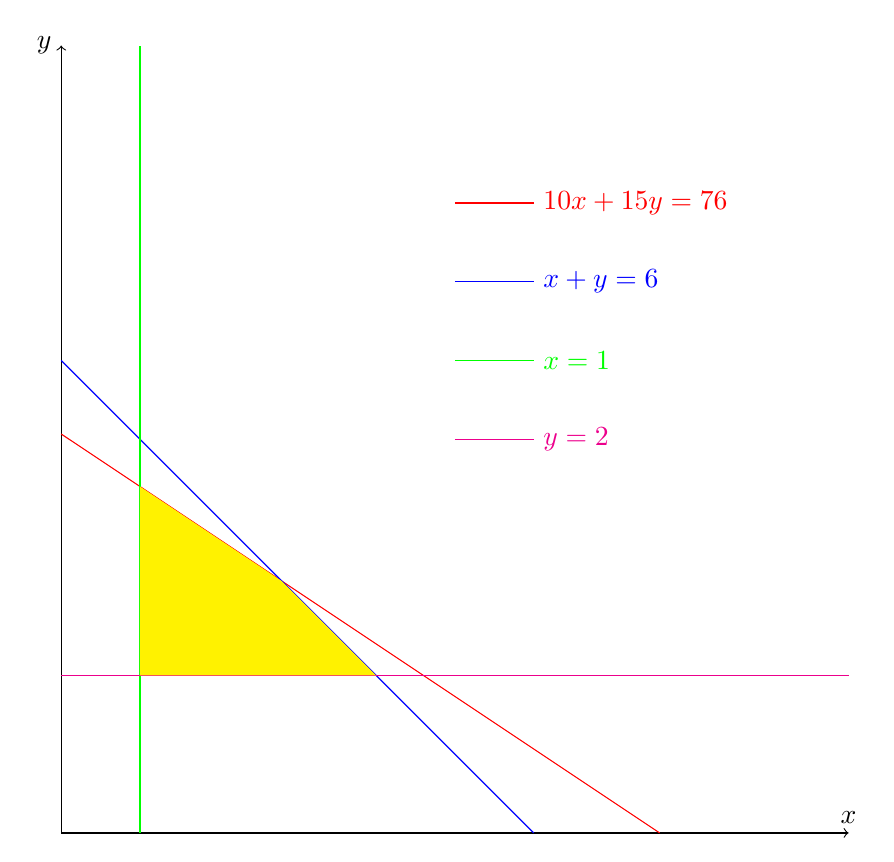
\begin{tikzpicture}
    \draw[->] (0,0) -- (10,0) node[above] {$x$};
    \draw[->] (0,0) -- (0,10) node[left] {$y$};
    \draw[color=red](0,5.066666666666666) -- (7.6,0);
    \draw[color=blue](0,6)--(6,0);
    \draw[color=green](1,0) --(1,10);
    \draw[color=magenta](0,2) --(10, 2);
    \draw[color=red] (5,8) --(6,8) node[right] {$10x+15y=76$};
    \draw[color=blue] (5,7) --(6,7) node[right] {$x+y=6$};
    \draw[color=green] (5,6) --(6,6) node[right] {$x=1$};
    \draw[color=magenta] (5,5) --(6,5) node[right] {$y=2$};
    \fill[color=yellow] (1,2) -- (1,4.4) -- (2.8,3.2) -- (4,2) -- cycle;
  \end{tikzpicture}
\end{center}

The accepted area is thus the content of the polygon in yellow delimited
by the points $(1,2)$, $\left(1,\frac{22}{5}\right)$,
$\left(\frac{14}{5},\frac{16}{5}\right)$ and $(4,2)$.

\subsection*{Exercício 5}

\begin{enumerate}
\item We can write
  $y^2-4y+x^2-2x+2 = {(y - 2)}^2 - 4 + {(x-1)}^2 + - 1 + 2 =
  {(y - y_1)}^2 + {(x-x_1)}^2 - R^2$
  where $y_1=2,x_1=1,R = \sqrt{3}$. So this is uma circunferência
  of center $(x_1,y_1)$ and radius $R$.
\item A point of the intersection would satisfy
  $y = \frac{2}{3}x - 2$ and reinjecting in the circunferência equation,
  we obtain $13x^2 -66x+126=0$. The discriminant of this equation is
  $\Delta = 66^2 - 4\times13\times126 < 0$ so the circunferência and reta
  do not intersect.
\item A point of the intersection would satisfy
  $y = -x + 3 + \sqrt{3}$. Reinjecting in the circunferência equation,
  we obtain $x^2 -{(\sqrt{3}+2)}x + \sqrt{3}+1 = 0$.
  This has two solutions: $x=1$ and $x=\sqrt{3}+1$.
  Hence the reta intersects the circunferência at point
  $(1,2+\sqrt{3})$ and $(1+\sqrt{3}, 2)$.
\item A point of the intersection would satisfy
  $x = 1 - \sqrt{3}$. Reinjecting in the circunferência equation,
  we obtain $y^2-4y+4={(y-2)}^2=0$ which has a unique solution $y=2$.
  So the reta is tangent to the circunferência at point
  $(1 - \sqrt{3}, 2)$.
\end{enumerate}

\subsection*{Exercício 6}
\begin{enumerate}
\item The first is the circunferência of center $(5,3)$ and radius $1$.
  The second is the circunferência of center $(7,3)$ and radius $3$.
\item $2{(7-3)}x + 2{(3-3)}y + 5^2+3^2-1^2-3^2-7^2+3^2 = 4x - 16 = 0$
  So the radical axis has equation $x=4$.
\item For example injecting $x=4$ in $y^2-6y+x^2-10x+33=0$
  we find $0=y^2-6y+9={(y-3)}^2$ that is $y=3$. So the
  two circunferências are tangent at point $(4,3)$.
\item These are circunferências of center $(0,1)$ and radius $1$ and
  center $(2,3)$ and radius $\sqrt{5}$.
  The radical axis has equation $4y+4x-8=0$.
  Reinjecting $x = -y + 2$ in $y^2-2y+x^2=0$
  we find $y^2-3y+2=0$ that is $y=2$ or $y=1$.
  Finally the circunferências intersect at points $(0,2)$ and $(1,1)$.
\end{enumerate}

\subsection*{Exercício 7}

Identify the curves given by the following equations

\begin{enumerate}
\item It can be simplified to the equation of the vertical
  line $x = \frac{1}{2}$.
\item Hyperbola of center $(1,3)$ and parameters, axis parallel to
  the cartesian coordinate system and parameters $a=2$, $b=1$.
\item Circunferência of center $(7,5)$ and radius $\sqrt{67}$.
\item Ellipse of center $(0,1)$, axis parallel to
  the cartesian coordinate system and parameters $a=\frac{1}{3}$ and
  $b=7$.
\item We can write it $y = 2{(x+1)}^2+3$. It is a parabola of axis
  of symmetry the $x=-1$, vertex $(-1,3)$ and parameter $p=\frac{1}{8}$.
\item Note that this is the graph of the function $x \mapsto \frac{1}{x}$.
  The suggestion gives
  $x = \frac{u-v}{\sqrt{2}}$ and
  $y = \frac{u+v}{\sqrt{2}}$ and so $xy=1$ is equivalent to
  $\left(\frac{u}{\sqrt{2}}\right)^2 - \left(\frac{v}{\sqrt{2}}\right)^2 = 1$.
\end{enumerate}

\subsection*{Exercício 8}

\begin{enumerate}
\item We have $d x(t) - b y(t) = da - bc$ so
  so the points of the curve are on the reta of equation
  $dx - by + bc - ad = 0$. Conversely, given any point on that reta
  then we set $t = \frac{x-a}{b}$. We have $a+tb = x$ and
  $c + td = c + \frac{dx-da}{b} = \frac{by - bc}{b} = y$. So this
  parameteric definition corresponds to the reta of equation
  $dx - by + bc - ad = 0$.

\item We note that for all $t$,
  ${\frac{x(t)}{a}}^2 + {\frac{y(t)}{b}}^2 = \cos^2{t} + \sin^2{t} = 1$.
  So the points of the curve are on the ellipse with axis those of the
  cartesian coordinate system and parameters $a,b$.
  Conversely, let any point $(x,y)$ on the ellipse such that $x,y \geq 0$.
  We have $0 \leq y \leq b$ and so
  $t = \arccos\left(1 - \left(\frac{y}{b}\right)^2\right)$ is well-defined.
  Then $\sin^2{(t)} = 1 - \cos^2{(t)} = \left(\frac{y}{b}\right)^2$
  and $\cos^2{t} = 1 - \left(\frac{y}{b}\right)^2 =
  \left(\frac{x}{a}\right)^2$ that is
  $x = a{|\cos{t}|}$ and
  $y = b{|\sin{t}|}$. Considering the parameters
  $\pm t$ and $\pi \pm t$ we can obtain all the points of the ellipse.

\item We note that for all $t$,
  ${\frac{t(t)}{a}}^2 - {\frac{y(t)}{b}}^2 =
  \frac{{(e^{2t}+2+e^{-2t})}-{(e^{2t}-2+e^{-2t})}}{4} = \frac{4}{4}=1$
  So the points of the curve are on the hyperbola with axis those of the
  cartesian coordinate system and parameters $a,b$.
  Conversely, let any point $(x,y)$ on the hyperbola such that $x \geq 0$.
  In order to find $t$ such that $y = b \frac{e^t-e^{-t}}{2}$,
  we let $X=e^{t} > 0$. This is equivalent to
  $X^2 - \frac{2y}{b} X - 1 = 0$. We have $\Delta =
  4\left(\left(\frac{y}{b}\right)^2+1\right) = 4\left(\frac{x}{a}\right)^2 > 0$
  and so two solutions
%%
  $$e^t = X =
  {-\frac{y}{b} \pm \sqrt{\left(\frac{y}{b}\right)^2+1}} =
  {-\frac{y}{b} \pm \frac{x}{a}}$$
%%
  Only the positive one is acceptable and we set
  $t = \ln\left(-\frac{y}{b} + \frac{x}{a}\right)$.
  Then we obtain
  $b \frac{e^t-e^{-t}}{2} = y$ and
  $a \frac{e^t+e^{-t}}{2} = x$. Hence we obtain all the points on one branch
  of the hyperbola where $x > 0$. Moreover, since for all $t$ we have
  $x(t) > 0$, the other branch of the hyperbola is not part of the curve.
  Remark: $\cosh{t} = \frac{e^t+e^{-t}}{2}$
  $\sinh{t} = \frac{e^t-e^{-t}}{2}$ are called hyperbolic cosine and sine and
  they have similar properties as $\cos$ and $\sin$.

\item Here we have an obvious description of a parabola with parameter $p$,
  axis of symmetry the $x$-axis and vertex $(0,0)$. The equation is
  $y^2 = 4px$.

\end{enumerate}

